\documentclass[12pt]{article}

\usepackage{sbc-template}
\usepackage{graphicx}
\usepackage[utf8]{inputenc}
\usepackage[brazilian]{babel}
\usepackage{amsmath}
\usepackage{booktabs}
\usepackage{xurl}
\usepackage{placeins}


\title{Análise do Impacto de Runtimes Task-Based no Desempenho de Algoritmos de Álgebra Linear Densa}

\author{Matheus Augusto Tregnago}

\address{Instituto de Informática -- Universidade Federal do Rio Grande do Sul
  (UFRGS)
  \email{matregnago@inf.ufrgs.br}}

\begin{document}

\maketitle

\begin{resumo}
	Runtimes de escalonamento de tarefas como StarPU e PaRSEC abstraem a complexidade de plataformas heterogêneas, mas adotam estratégias diferentes de escalonamento e gerenciamento de dados. Este trabalho compara o desempenho dos dois runtimes nas fatorações de Cholesky e LU sem pivotamento da biblioteca Chameleon, mantendo fixa a biblioteca de álgebra linear para isolar o efeito do runtime, o que exigiu estender a interface de inserção dinâmica de tarefas do PaRSEC (DTD) e os codelets do Chameleon com suporte a GPU. Os experimentos, executados nas partições tupi e poti do cluster PCAD \footnote{https://pcad.inf.ufrgs.br/}, mostram que nenhum runtime é sistematicamente superior: na poti, cuja GPU é fraca em precisão dupla, o PaRSEC com o escalonador \texttt{gd} vence por tratar a GPU como recurso acessório; na tupi, cuja GPU é forte, o StarPU vence com folga por ocupá-la de forma mais eficiente.
\end{resumo}

\section{Introdução}

Nos últimos anos, as arquiteturas de computação de alto desempenho têm se tornado cada vez mais heterogêneas, combinando processadores multicore convencionais com aceleradores especializados, como GPUs, FPGAs e outros aceleradores. Essa diversidade de tecnologias, somada às diferenças entre os modelos de execução e as hierarquias de memória, torna difícil programar essas plataformas de forma eficiente. Nesse modelo, uma aplicação é decomposta em tarefas com dependências de dados explícitas, o que permite escalonar sua execução de forma dinâmica, conforme os recursos disponíveis \cite{10025520}.

Para facilitar o uso desse paradigma, diversos runtimes de escalonamento de tarefas foram criados para mapear as tarefas de uma aplicação para os recursos computacionais disponíveis, de forma transparente ao programador. Esses sistemas decidem quando e onde cada tarefa será executada, gerenciam as transferências de dados necessárias entre as diferentes unidades de processamento e memórias e equilibram a carga de trabalho entre os recursos, tanto em ambientes de memória compartilhada quanto em ambientes distribuídos \cite{aguerrebere2018hdr}.

StarPU \cite{starpu} é um desses runtimes. Nele, o desenvolvedor pode fornecer diferentes implementações para uma mesma tarefa, uma para CPU e outra para GPU, por exemplo, e deixar que o próprio ambiente de execução selecione automaticamente a implementação mais adequada, considerando o ambiente computacional e a disponibilidade de recursos, buscando otimizar o desempenho. Isso isola o desenvolvedor dos detalhes da arquitetura de destino, permitindo criar aplicações mais simples e fáceis de escalar.

PaRSEC \cite{bosilca2011dague} é outro desses runtimes, com foco em ambientes de memória distribuída compostos por múltiplos nós multicore, possivelmente equipados com aceleradores. Diferentemente de abordagens que constroem o DAG completo da aplicação em memória antes de escaloná-lo, o PaRSEC representa as dependências entre tarefas de forma compacta e simbólica, o que lhe permite escalar para milhões de tarefas com baixo overhead e favorecer, de forma totalmente distribuída, tanto o balanceamento de carga quanto a sobreposição entre computação e comunicação.

Embora StarPU e PaRSEC compartilhem o mesmo objetivo de abstrair o escalonamento de tarefas em plataformas heterogêneas, cada um adota estratégias diferentes de escalonamento e de gerenciamento de comunicações, o que pode impactar bastante o desempenho de algoritmos de álgebra linear densa.

Para conduzir essa avaliação, este trabalho utiliza o Chameleon \cite{AGULLO2012473}, uma biblioteca de álgebra linear densa que implementa fatorações como LU, Cholesky e QR por meio de algoritmos por blocos \cite{DBLP}, delegando o escalonamento de suas tarefas a um runtime externo, como o StarPU e o PaRSEC.

Os experimentos foram executados em duas partições do cluster PCAD, no INF/UFRGS: (i) tupi, equipada com um processador Intel Core i9-14900KF (24 núcleos físicos, 3,2 GHz) e uma GPU NVIDIA GeForce RTX 4090 (24 GB); (ii) poti, equipada com um processador Intel Core i7-14700KF (20 núcleos físicos, 3,4 GHz) e uma GPU NVIDIA GeForce RTX 4070 (12 GB).

Os resultados dos experimentos mostraram que nenhum dos dois runtimes é sistematicamente superior ao outro: na partição poti, cuja GPU é fraca em precisão dupla, o PaRSEC com o escalonador \texttt{gd} superou o StarPU por usar a GPU como recurso acessório e não impor custo sobre os workers de CPU; na partição tupi, cuja GPU é forte, o StarPU venceu com folga graças a maior ocupação da GPU.

O restante deste trabalho está organizado da seguinte forma. A Seção 2 apresenta os trabalhos relacionados. A Seção 3 descreve os conceitos utilizados neste trabalho, enquanto a Seção 4 apresenta as soluções desenvolvidas. A Seção 5 detalha nossa metodologia experimental, seguida pelos resultados experimentais na Seção 6. Por fim, a Seção 7 conclui este trabalho.

\section{Trabalhos Relacionados}

Diversos trabalhos avaliam runtimes task-based aplicados a algoritmos de álgebra linear densa, mas cada um deles isola apenas parte do problema, limitando a comparação a um único runtime ou comparando runtimes distintos por meio de bibliotecas de álgebra linear diferentes.

Hoque et al. \cite{10.1145/3148226.3148233} comparam os dois paradigmas de programação oferecidos pelo PaRSEC: o Parameterized Task Graph (PTG) e o Dynamic Task Discovery (DTD) utilizando o Chameleon em conjunto com PaRSEC, StarPU e QUARK. A avaliação, no entanto, é restrita a execuções somente em CPU, sem considerar aceleradores.

Lisito et al. \cite{11078555} avaliam a fatoração LU com pivotamento parcial, comparando o StarPU (com o Chameleon) e o PaRSEC (com o DPLASMA). Como cada runtime é avaliado em conjunto com uma biblioteca de álgebra linear diferente, eventuais diferenças de desempenho observadas podem ser atribuídas tanto ao runtime quanto à implementação específica de cada biblioteca.

Agullo et al. \cite{7284288} comparam o desempenho da fatoração de Cholesky sobre o StarPU com limites teóricos de desempenho em plataformas heterogêneas. O trabalho, contudo, considera apenas o StarPU, sem comparação direta com outro runtime de escalonamento de tarefas.

Não foi encontrado nenhum trabalho anterior que compara StarPU e PaRSEC utilizando a mesma biblioteca de álgebra linear densa em um ambiente heterogêneo. Esse é o diferencial deste trabalho, no qual foi fixado o Chameleon como biblioteca única e variado apenas o runtime e o escalonador utilizado.

\section{Fundamentação Teórica}
Nesta seção, apresentamos uma visão geral dos runtimes de escalonamento de tarefas, StarPU e PaRSEC, e da biblioteca de álgebra linear densa Chameleon utilizados neste trabalho.
\subsection{StarPU}

StarPU \cite{starpu} é um framework escrito em C para programação orientada a tarefas em plataformas híbridas compostas por CPUs e GPUs. As tarefas de uma aplicação StarPU são definidas por meio de codelets, estruturas que agrupam uma ou mais implementações de uma mesma operação, além da forma como cada um de seus parâmetros é acessado. A partir da ordem de submissão das tarefas e dos modos de acesso declarados para cada dado, o StarPU constrói implicitamente um grafo acíclico dirigido (DAG) de dependências, sem que o programador precise expressá-lo manualmente. Em tempo de execução, o runtime escolhe qual das implementações disponíveis será utilizada para cada tarefa, considerando a disponibilidade dos recursos, a distribuição de carga entre os workers e o custo das cópias de dados envolvidas. O gerenciamento de memória nos aceleradores também é responsabilidade do StarPU, que realiza alocação e liberação de buffers na GPU, cópias entre a memória do host e do dispositivo, e a sobreposição dessas transferências com a computação por meio de prefetching.

\subsection{PaRSEC}

PaRSEC \cite{bosilca2011dague} é um framework para escalonamento de tarefas voltado a ambientes de memória distribuída compostos por múltiplos nós multicore. Diferentemente de runtimes que desenrolam o DAG completo da aplicação em memória antes de escaloná-lo, o PaRSEC representa o grafo de dependências de forma compacta e simbólica, por meio de um formato conhecido como Parameterized Task Graph (PTG), também chamado de Job Data Flow (JDF). O escalonamento é totalmente distribuído, cada nó executa sua própria instância do escalonador, que utiliza filas locais por thread e mecanismos de furto de trabalho sensíveis à hierarquia NUMA para favorecer o reaproveitamento de cache. As comunicações entre nós são implícitas, inferidas diretamente das dependências de dados do grafo, e são tratadas de forma assíncrona por uma thread dedicada, permitindo a sobreposição entre computação e comunicação. Assim como o StarPU, o PaRSEC também oferece suporte a aceleradores por meio de múltiplas implementações para uma mesma tarefa, permitindo que o escalonador decida em tempo de execução em qual unidade.

\subsection{Chameleon}

Chameleon \cite{AGULLO2012473} é uma biblioteca escrita em C que fornece rotinas para a resolução de sistemas lineares gerais densos, sistemas simétricos positivos definidos e problemas de mínimos quadrados lineares, por meio das fatorações LU, Cholesky, QR e LQ. Assim como as bibliotecas PLASMA e MAGMA, o Chameleon segue a abordagem de algoritmos por blocos \cite{DBLP}, em que cada fatoração é decomposta em uma sequência de tarefas de granularidade fina que operam sobre submatrizes quadradas, reduzindo a necessidade de sincronizações globais e expondo um grau de paralelismo bem maior do que o obtido pelas versões tradicionais orientadas a blocos de linha/coluna, como as do LAPACK e do ScaLAPACK. A fatoração de Cholesky por tiles, por exemplo, é expressa como uma sequência de chamadas às rotinas POTRF, TRSM, SYRK e GEMM, cada uma correspondendo a uma tarefa cujas dependências de dados definem um DAG. Em vez de escalonar essas tarefas de forma estática, o Chameleon delega essa responsabilidade a um runtime de escalonamento de tarefas, como o StarPU, o PaRSEC ou o OpenMP, enquanto a implementação interna de cada tarefa reutiliza rotinas clássicas de BLAS e LAPACK. Essa separação entre a descrição do algoritmo, em termos de tarefas e dependências, e sua execução propriamente dita é o que permite ao Chameleon explorar arquiteturas heterogêneas compostas por CPUs e GPUs sem que o algoritmo precise ser reescrito para cada plataforma. Neste trabalho, o Chameleon é utilizado em conjunto com os runtimes StarPU e PaRSEC para executar as fatorações Cholesky e LU sem pivotamento em um nó heterogêneo por vez, nas partições tupi e poti do cluster PCAD.

Ao longo deste trabalho, identificamos que a comparação entre StarPU e PaRSEC não era diretamente possível a partir das versões atuais disponíveis do Chameleon e do PaRSEC, pois, enquanto os codelets do Chameleon para o StarPU já possuem suporte maduro a GPU, a interface de inserção dinâmica de tarefas do PaRSEC (DTD) não suportava a execução de tarefas em GPU, e os codelets do Chameleon para o PaRSEC estavam limitados à CPU. A seção a seguir descreve as principais modificações que desenvolvemos no PaRSEC e no Chameleon para permitir essa comparação.

\section{Soluções desenvolvidas}

A interface DTD do PaRSEC permitia associar a cada tarefa apenas uma implementação em CPU, diferentemente da interface estática PTG, que já suporta múltiplas implementações por tarefa. Adicionamos ao PaRSEC uma nova função, que permite registrar, além da implementação em CPU, uma implementação em GPU para a mesma tarefa. Em tempo de execução, o escalonador passa a tentar primeiro a implementação em GPU, delegando a submissão ao mesmo mecanismo de escalonamento de GPU já utilizado pelo backend PTG, usando a implementação em CPU apenas quando nenhum dispositivo está disponível.

Essa mudança expôs um problema de coerência de dados: quando uma tarefa executada em CPU escrevia um tile, o caminho de execução da DTD não invalidava corretamente eventuais cópias desse tile já presentes na memória da GPU. Uma tarefa de GPU subsequente podia então ler dados desatualizados, produzindo resultados numericamente incorretos. Corrigimos o problema invalidando explicitamente as cópias de dispositivo de um tile sempre que uma tarefa de CPU o modifica.

Com o suporte a GPU já disponível na interface DTD do PaRSEC, implementamos, no lado do Chameleon, as implementações em GPU dos codelets utilizados pelas fatorações avaliadas neste trabalho, que até então só possuíam implementação em CPU quando executadas com o PaRSEC. Cada uma dessas implementações delega o cálculo às bibliotecas cuBLAS e cuSOLVER, de forma análoga aos codelets equivalentes já existentes para o StarPU, associando-as à sua contraparte de CPU por meio da nova função de inserção de tarefas com suporte a CUDA.


\section{Metodologia}
Nesta seção, apresentamos nossa metodologia experimental. Primeiro, damos uma visão geral das aplicações de álgebra linear densa consideradas neste estudo, depois, descrevemos o ambiente de execução utilizado nos experimentos e, por fim, detalhamos o projeto experimental adotado.
\subsection{Aplicações}

Consideramos dois algoritmos de fatorações disponíveis no Chameleon: a fatoração de Cholesky e a fatoração LU sem pivotamento.

A fatoração de Cholesky (\texttt{potrf}) decompõe uma matriz real simétrica positiva definida $A$, de ordem $n \times n$, na forma $A = LL^T$, em que $L$ é uma matriz real triangular inferior de ordem $n \times n$ com elementos diagonais positivos. O algoritmo por tiles utiliza quatro tipos de tarefa: POTRF, SYRK, TRSM e GEMM. A tarefa POTRF, executada sobre os tiles da diagonal, possui apenas implementação em CPU, enquanto as demais possuem implementações em CPU e em GPU.

A fatoração LU sem pivotamento (\texttt{getrf\_nopiv}) decompõe uma matriz real $A$, de ordem $n \times n$, na forma $A = LU$, em que $L$ é triangular inferior e $U$ é triangular superior. O projeto desse algoritmo por tiles para sistemas acelerados por GPU é descrito por Agullo et al. \cite{6126599}. O algoritmo utiliza três tipos de tarefa: GETRF, TRSM e GEMM. A tarefa GETRF, que fatora o tile da diagonal, possui apenas implementação em CPU, enquanto TRSM e GEMM possuem implementações em CPU e em GPU.

\subsection{Ambiente de Execução}

Utilizamos duas partições do cluster PCAD, no INF/UFRGS, nos experimentos: tupi e poti. A Tabela~\ref{tab:hw} especifica o hardware de cada partição.

\begin{table}[h]
	\centering
	\caption{Especificação de hardware das partições utilizadas.}
	\label{tab:hw}
	\begin{tabular}{@{}lllll@{}}
		\toprule
		Partição & CPU                   & RAM    & GPU             & Armazenamento \\
		\midrule
		tupi     & Intel Core i9-14900KF & 128 GB & NVIDIA RTX 4090 & 1,8 TB NVMe   \\
		         & 3,2 GHz, 24 núcleos   &        & 24 GB           &               \\
		poti     & Intel Core i7-14700KF & 96 GB  & NVIDIA RTX 4070 & 119,2 GB NVMe \\
		         & 3,4 GHz, 20 núcleos   &        & 12 GB           & + 1,7 TB SSD  \\
		\bottomrule
	\end{tabular}
\end{table}

Do ponto de vista de software, utilizamos o Chameleon na versão 1.4.0, com suporte a CUDA habilitado. Como runtimes de escalonamento, utilizamos o StarPU e uma versão do PaRSEC derivada de um fork mantido por desenvolvedores do próprio Chameleon, ambos também compilados com suporte a CUDA e com a coleta de rastros de execução habilitada. A reprodutibilidade de todo o ambiente é garantida por meio do gerenciador de pacotes Nix, com as dependências fixadas em um flake.

A análise dos dados é realizada após a execução por meio de scripts escritos na linguagem R, utilizando o framework StarVZ \cite{Pinto2021ProvidingIP} para a visualização dos rastros de execução coletados pelo StarPU e pelo PaRSEC.

\subsection{Projeto Experimental}

Realizamos três projetos experimentais para investigar a influência do escalonador, do tamanho do problema e da máquina alvo no desempenho das fatorações Cholesky (potrf) e LU sem pivotamento (getrf\_nopiv), medido em GFLOPS. Em todos eles, o GFLOPS relatado pela própria aplicação é a variável de resposta.

Nosso estudo preliminar tem como objetivo determinar o tamanho de tile ideal para cada máquina, por meio de uma varredura sistemática de configurações de tile em precisão dupla. Fixamos o tamanho da matriz de entrada em $N=40.000$ com precisão dupla e variamos o tamanho do tile dentro de um conjunto de valores. Cruzamos essas configurações com as duas fatorações (\texttt{potrf}, \texttt{getrf\_nopiv}) e quatro combinações de runtime e escalonador: StarPU com \texttt{dmda} e \texttt{dmdas}; PaRSEC com \texttt{lfq} e \texttt{gd}. Além disso, executamos o mesmo desenho experimental em ambas as partições do PCAD, tupi e poti, variando apenas o número de threads de acordo com o número de núcleos físicos disponíveis em cada uma. A ordem de execução foi aleatorizada, com cinco repetições por configuração. O pico de GFLOPS observado em cada máquina, em precisão dupla, determina o tamanho de tile utilizado nas duas etapas seguintes. Os valores escolhidos foram $b=1.000$ na tupi, e $b=500$ na poti.

Nosso projeto fatorial completo investiga os efeitos de interação entre três fatores que influenciam o desempenho das fatorações em precisão dupla: a máquina utilizada (tupi ou poti), a combinação de runtime e escalonador e o tamanho do problema, fixando o tamanho de tile no valor ótimo identificado para cada máquina na etapa anterior. Como esse valor de tile determina a granularidade computacional disponível para cada GPU, o intervalo de valores de N explorado também foi definido por máquina: dez níveis entre 5.000 e 60.000 na tupi, e seis níveis entre 5.000 e 60.000 na poti. Para cada uma das duas fatorações, executamos todas as combinações desse desenho fatorial em ordem aleatorizada, com três repetições na tupi e cinco na poti.

Por fim, a terceira etapa emprega os mecanismos de coleta de rastros de execução do StarPU e do PaRSEC para realizar uma análise detalhada de desempenho, por meio de oito execuções representativas por máquina, sem repetições. Fixamos o tamanho da matriz em $N=40.000$ e o tamanho de tile no valor ótimo de cada máquina, variando as duas fatorações e as quatro combinações de runtime e escalonador. Fizemos essa análise com o auxílio do StarVZ \cite{Pinto2021ProvidingIP}.

\section{Resultados}

\subsection{Escolha do tamanho de tile}

A Figura~\ref{fig:gflops-b} mostra o resultado da varredura de tamanho de tile para as quatro combinações de runtime e escalonador em precisão dupla, com $N=40.000$ fixo em cada máquina.

\begin{figure}[h]
	\centering
	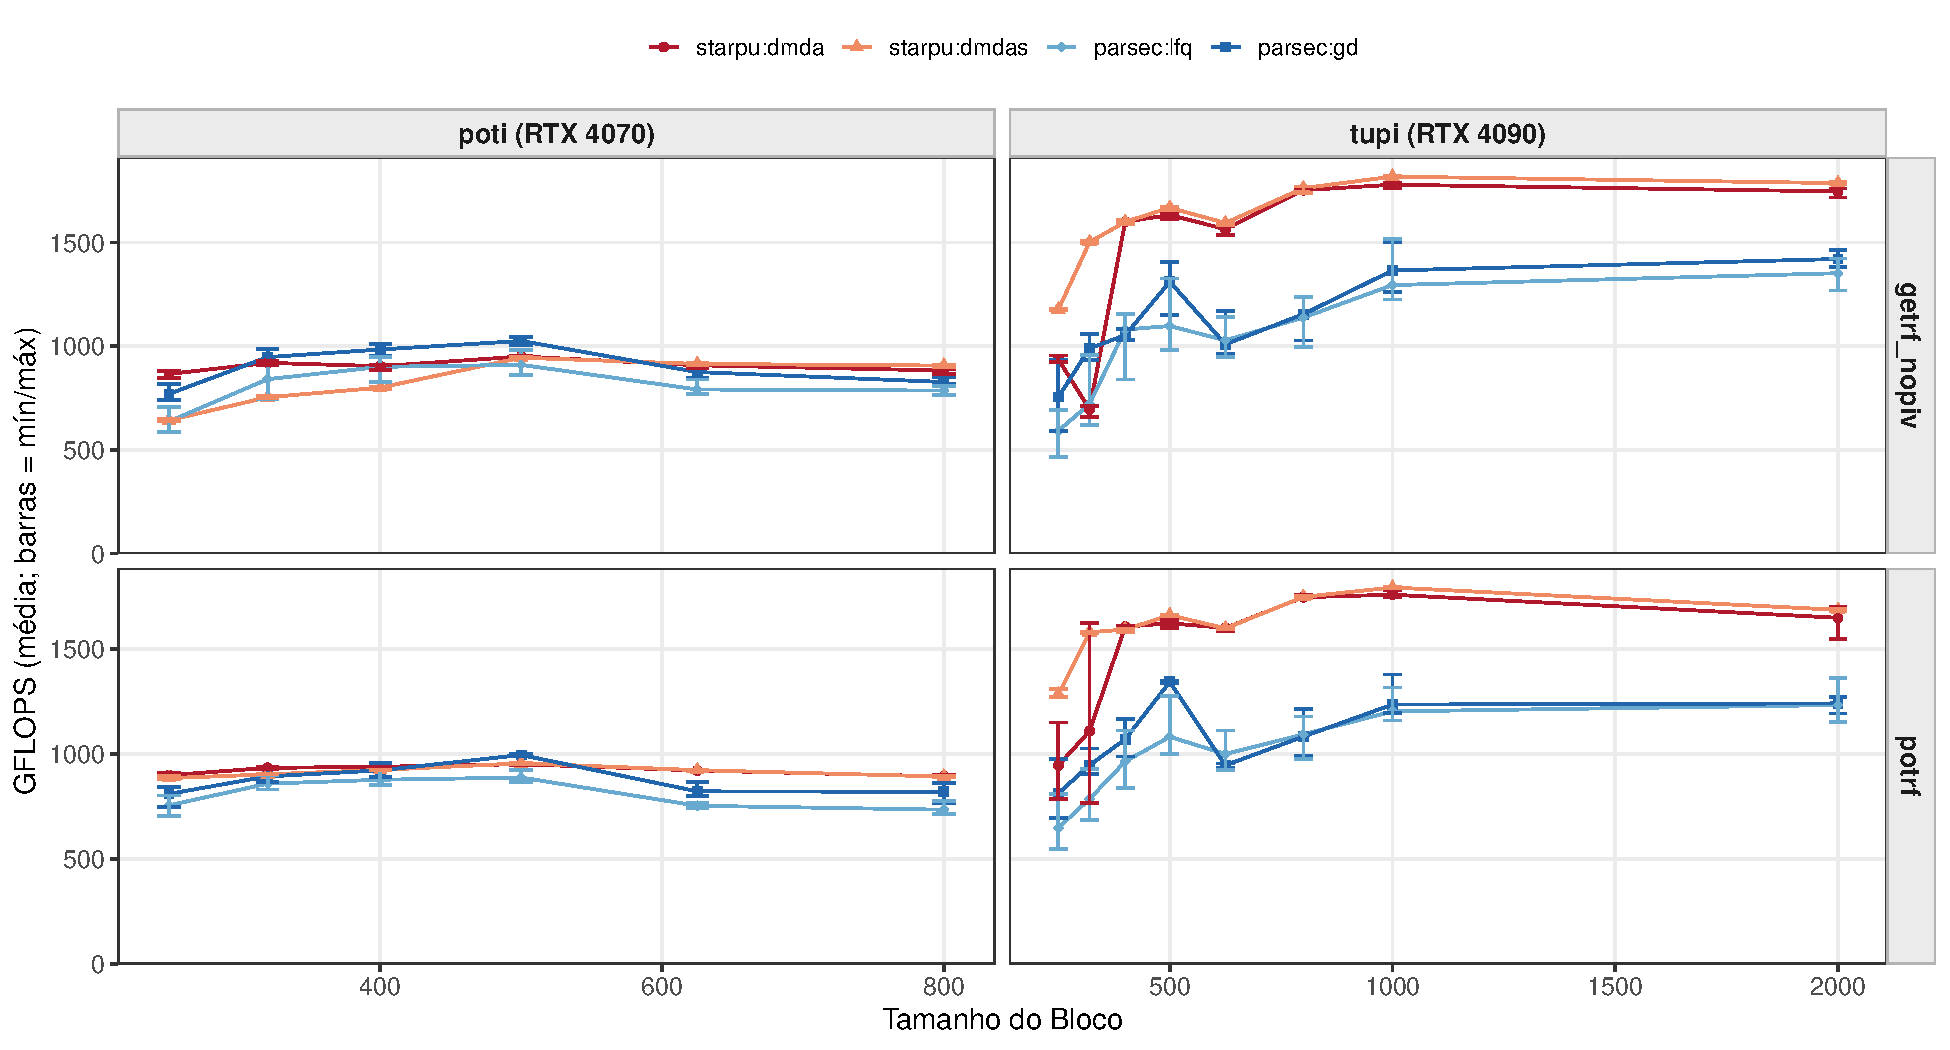
\includegraphics[width=\linewidth]{../plots/final/gflops_vs_b_compare.pdf}
	\caption{GFLOPS em função do tamanho de tile $b$, por algoritmo e
		máquina. }
	\label{fig:gflops-b}
\end{figure}

Na poti, as quatro configurações convergem para um pico em torno de $b=500$. Na tupi, por outro lado, há uma divergência estrutural entre os dois runtimes: o StarPU tem o seu pico em $b=1.000$, enquanto o PaRSEC só atinge seu melhor resultado em $b=2.000$ e cai mais acentuadamente para tiles menores ou maiores que o seu próprio ótimo.

\subsection{Desempenho em função do tamanho do problema}

A Figura~\ref{fig:gflops-n} apresenta o resultado do projeto fatorial completo.

\begin{figure}[h]
	\centering
	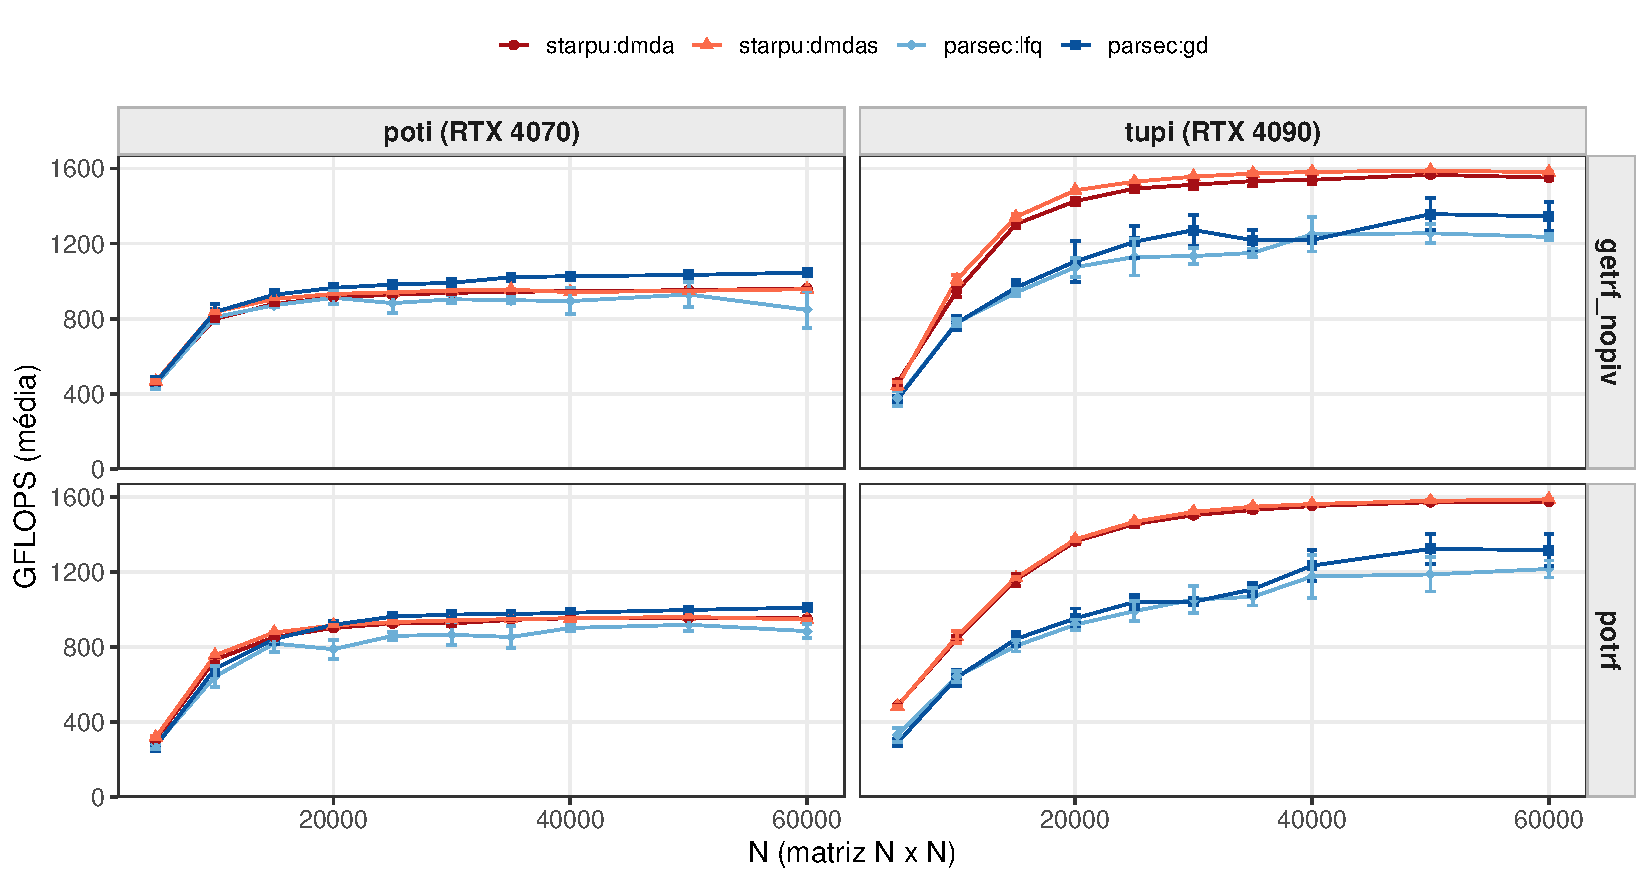
\includegraphics[width=\linewidth]{../plots/final/gflops_vs_n_compare.pdf}
	\caption{GFLOPS médio em função de $N$, por algoritmo e máquina.}
	\label{fig:gflops-n}
\end{figure}

O padrão que aparece na Figura~\ref{fig:gflops-n} é a observação central que organiza o restante desta seção. Na poti, o StarPU lidera até $N\approx10.000$, mas a partir de $N\approx20.000$ o \texttt{parsec:gd} assume a liderança e a mantém até $N=60.000$, o maior valor testado. Na tupi, por sua vez, o StarPU lidera em toda a faixa de $N$, com a vantagem sobre o PaRSEC aumentando à medida que $N$ cresce. Esse resultado contraria a intuição de que o StarPU, por manter um modelo de desempenho aprendido em tempo de execução, deveria vencer sistematicamente o PaRSEC, que decide o escalonamento de GPU de forma estática, sem medir tempos reais de execução. A próxima seção usa os rastros de execução coletados nas configurações de $N=40.000$ para explicar por que o resultado se inverte entre as duas máquinas.

\subsection{Análise de rastros de execução}
Para entender a inversão observada na seção anterior, analisamos em detalhe os rastros de execução coletados para a fatoração de Cholesky com $N=40.000$ e o tile ideal de cada máquina.

O ponto de partida é a diferença de capacidade das duas GPUs em precisão dupla. A RTX 4070 da poti tem pico teórico de apenas 458 GFLOPS em FP64, um valor abaixo da capacidade agregada dos 20 núcleos de CPU do nó, enquanto a RTX 4090 da tupi tem pico de aproximadamente 1,3 TFLOPS, muito acima da capacidade da CPU da tupi.

A Figura~\ref{fig:gpu-split} mostra o efeito dessa divisão sobre o desempenho total na poti, decompondo o GFLOPS entregue por cada classe de recurso. Na poti, a melhor estratégia é usar a GPU como recurso à parte, e é exatamente isso que o \texttt{gd} faz, porque sua fila global simples não introduz custo estrutural sobre os workers de CPU.

\begin{figure}[h]
	\centering
	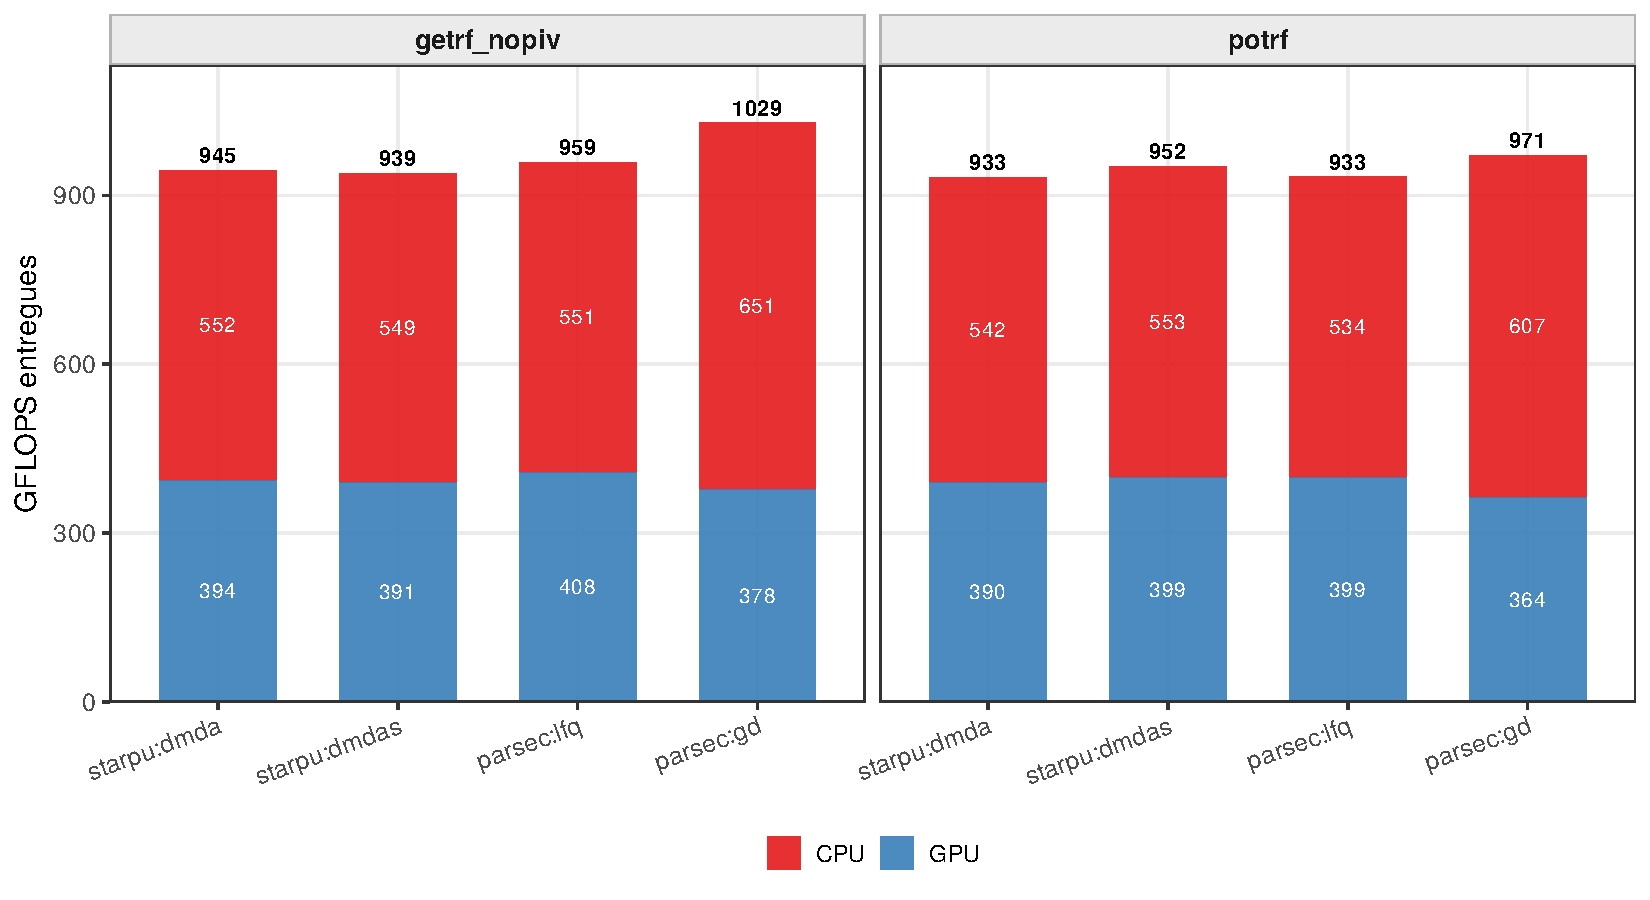
\includegraphics[width=\linewidth]{../plots/final/why_gd_poti/gpu_split_contrib.pdf}
	\caption{GFLOPS entregues por classe de recurso (CPU/GPU) na poti, por
		algoritmo e configuração.}
	\label{fig:gpu-split}
\end{figure}

Duas assimetrias, uma em cada lado, explicam o resultado da poti. Do lado da CPU, a tarefa \texttt{gemm} custa cerca de 26\% mais no StarPU do que no PaRSEC, pois o StarPU dedica quatro threads de worker à gestão da GPU, que disputam os mesmos núcleos físicos usados pelos workers de CPU comuns. Por outro lado, o PaRSEC gerencia a GPU sem thread dedicada, e por isso seus workers de CPU rendem mais por segundo ocupado. Do lado da GPU, porém, a tarefa \texttt{gemm} executa 2,9 vezes mais rápido no StarPU do que no PaRSEC na poti e cerca de 3 vezes mais rápido na tupi. O prefetching e o pipelining entre as fases de H2D, execução e D2H do StarPU tornam sua execução de GPU mais eficiente por tarefa em qualquer uma das duas máquinas.

\subsubsection{Painéis espaço-tempo e progressão do DAG}

A Figura~\ref{fig:st-compare} mostra os painéis espaço-tempo das quatro configurações na poti. O StarPU usa quatro \emph{lanes} de GPU dedicadas, sempre ocupadas por \texttt{gemm} do início ao fim da execução. Já o PaRSEC usa seis \emph{lanes} de \emph{stream}: duas reservadas a transferências H2D/D2H e quatro de execução. Essas quatro \emph{streams} de execução são visivelmente menos ocupadas, o que é uma evidência visual do menor uso da GPU pelo PaRSEC discutido na seção anterior. As faixas de workers de CPU, por sua vez, aparecem igualmente saturadas nas quatro configurações.

\begin{figure}[h]
	\centering
	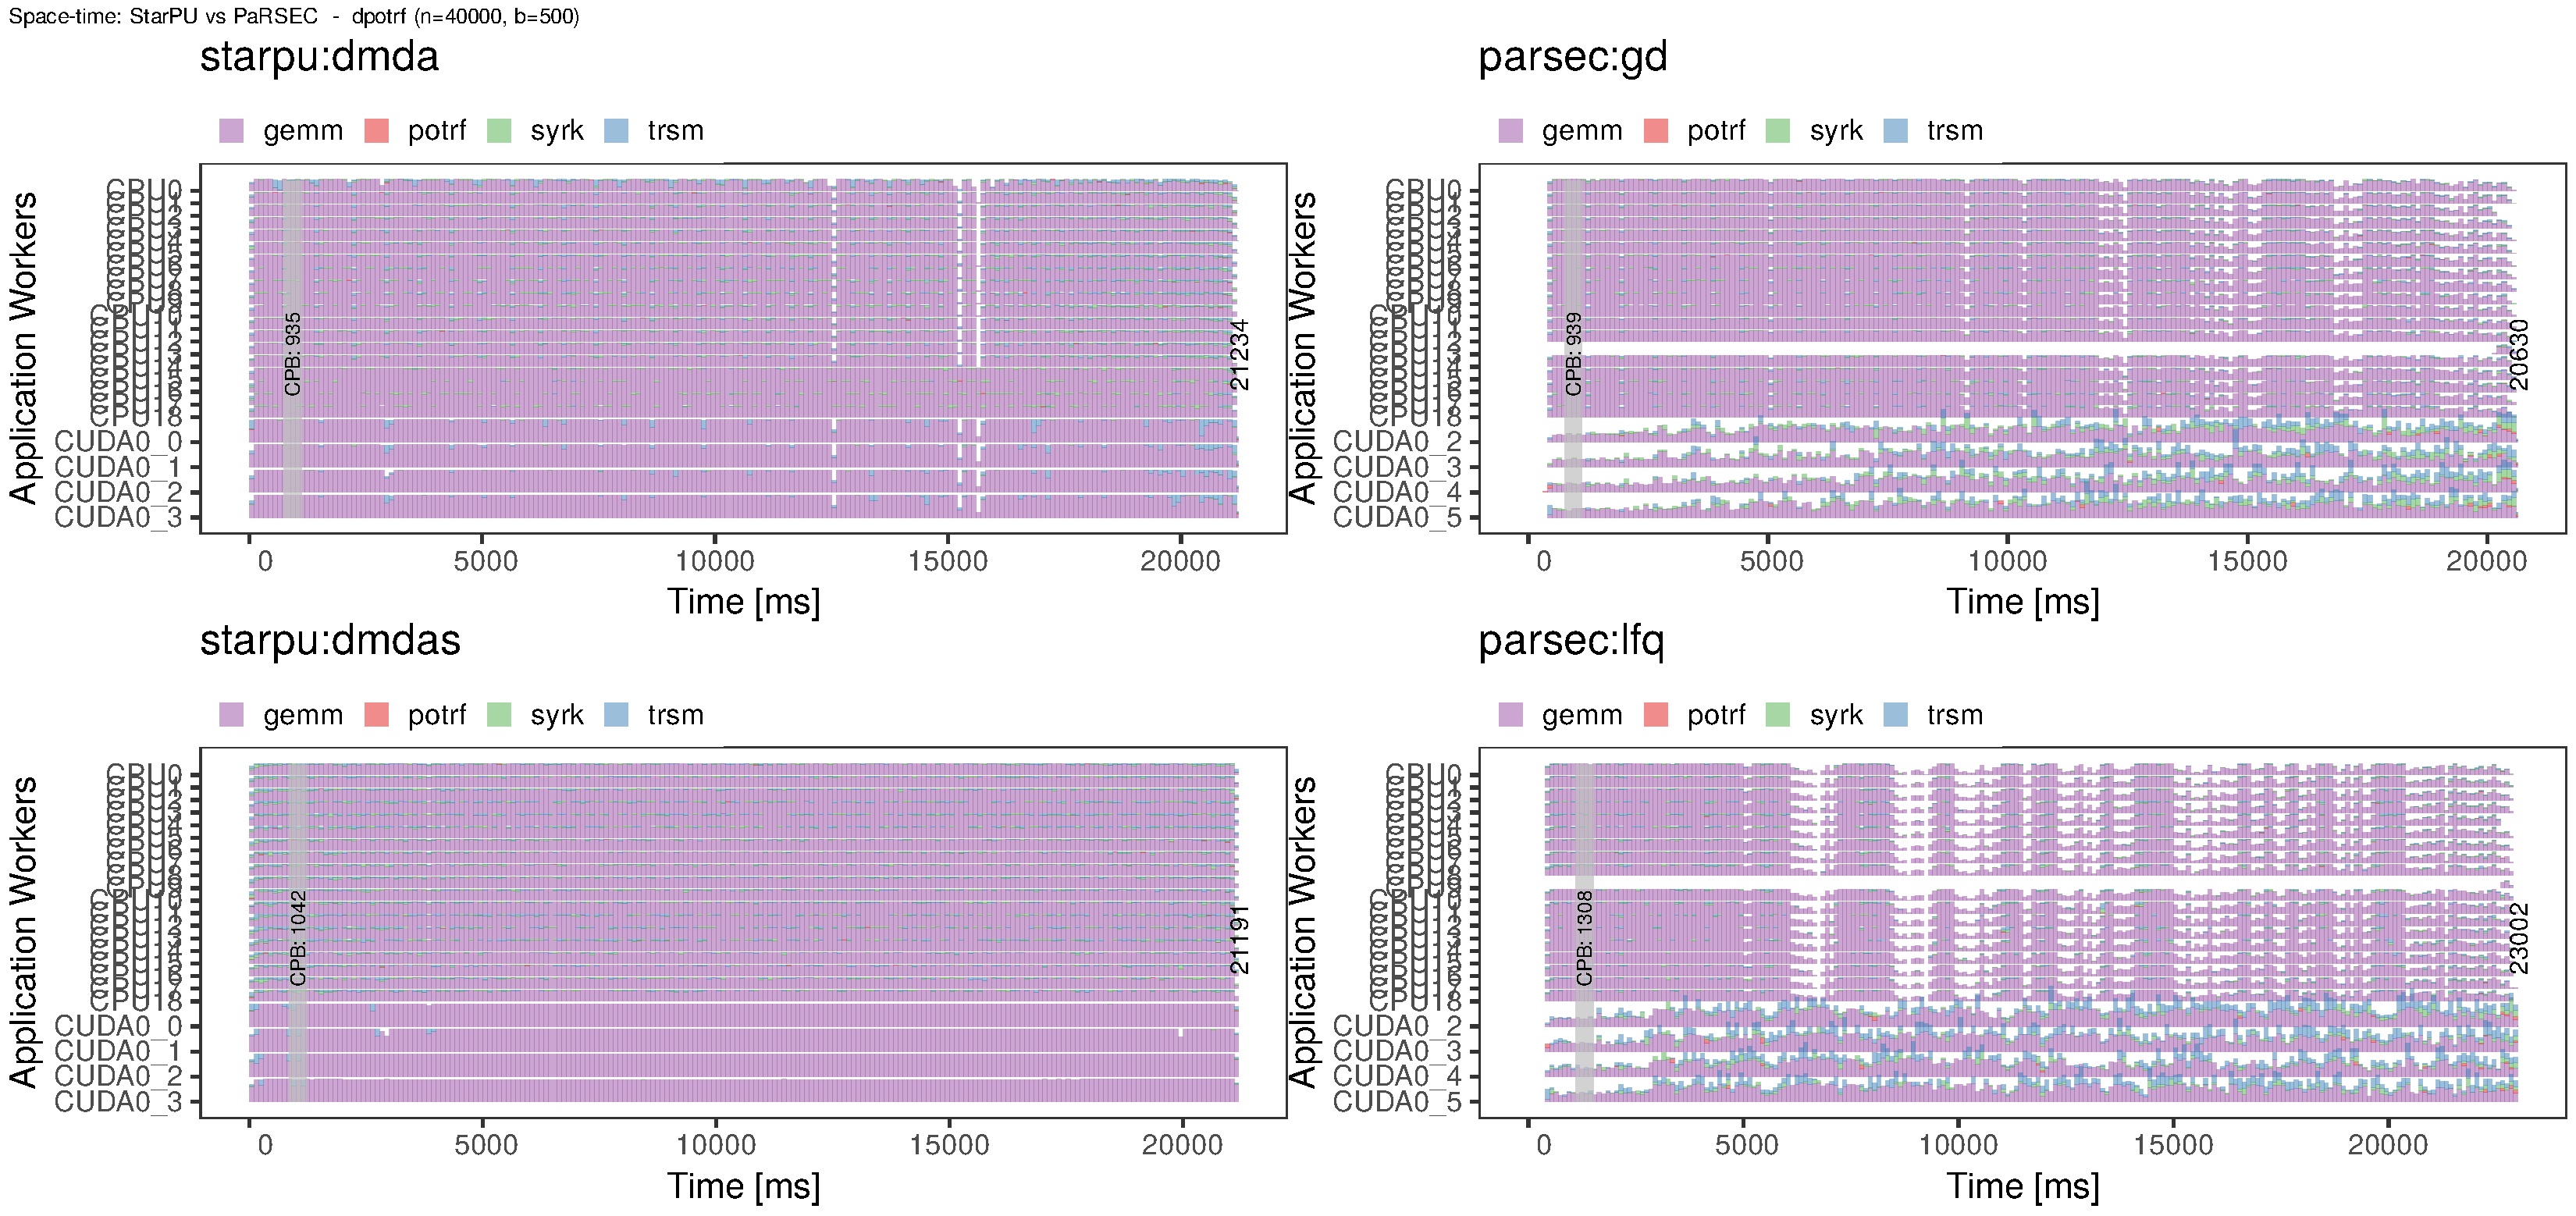
\includegraphics[width=\linewidth]{../plots/final/gpu_traces_poti_20260701_131857/st_compare_dpotrf.pdf}
	\caption{Painéis espaço-tempo de StarPU e PaRSEC na poti.}
	\label{fig:st-compare}
\end{figure}

A Figura~\ref{fig:kiteration} mostra a progressão da fatoração ao longo de suas iterações em função do tempo. O \texttt{dmda} progride de forma quase linear. O \texttt{dmdas} mostra uma dispersão, o que significa que sua política de priorização pelo caminho crítico adianta a execução de tarefas de iterações futuras. Já o \texttt{gd} e o \texttt{lfq} progridem de forma irregular, por conta da ausência de um modelo de desempenho guiando a ordem de despacho das tarefas para a GPU no PaRSEC.

\begin{figure}[h]
	\centering
	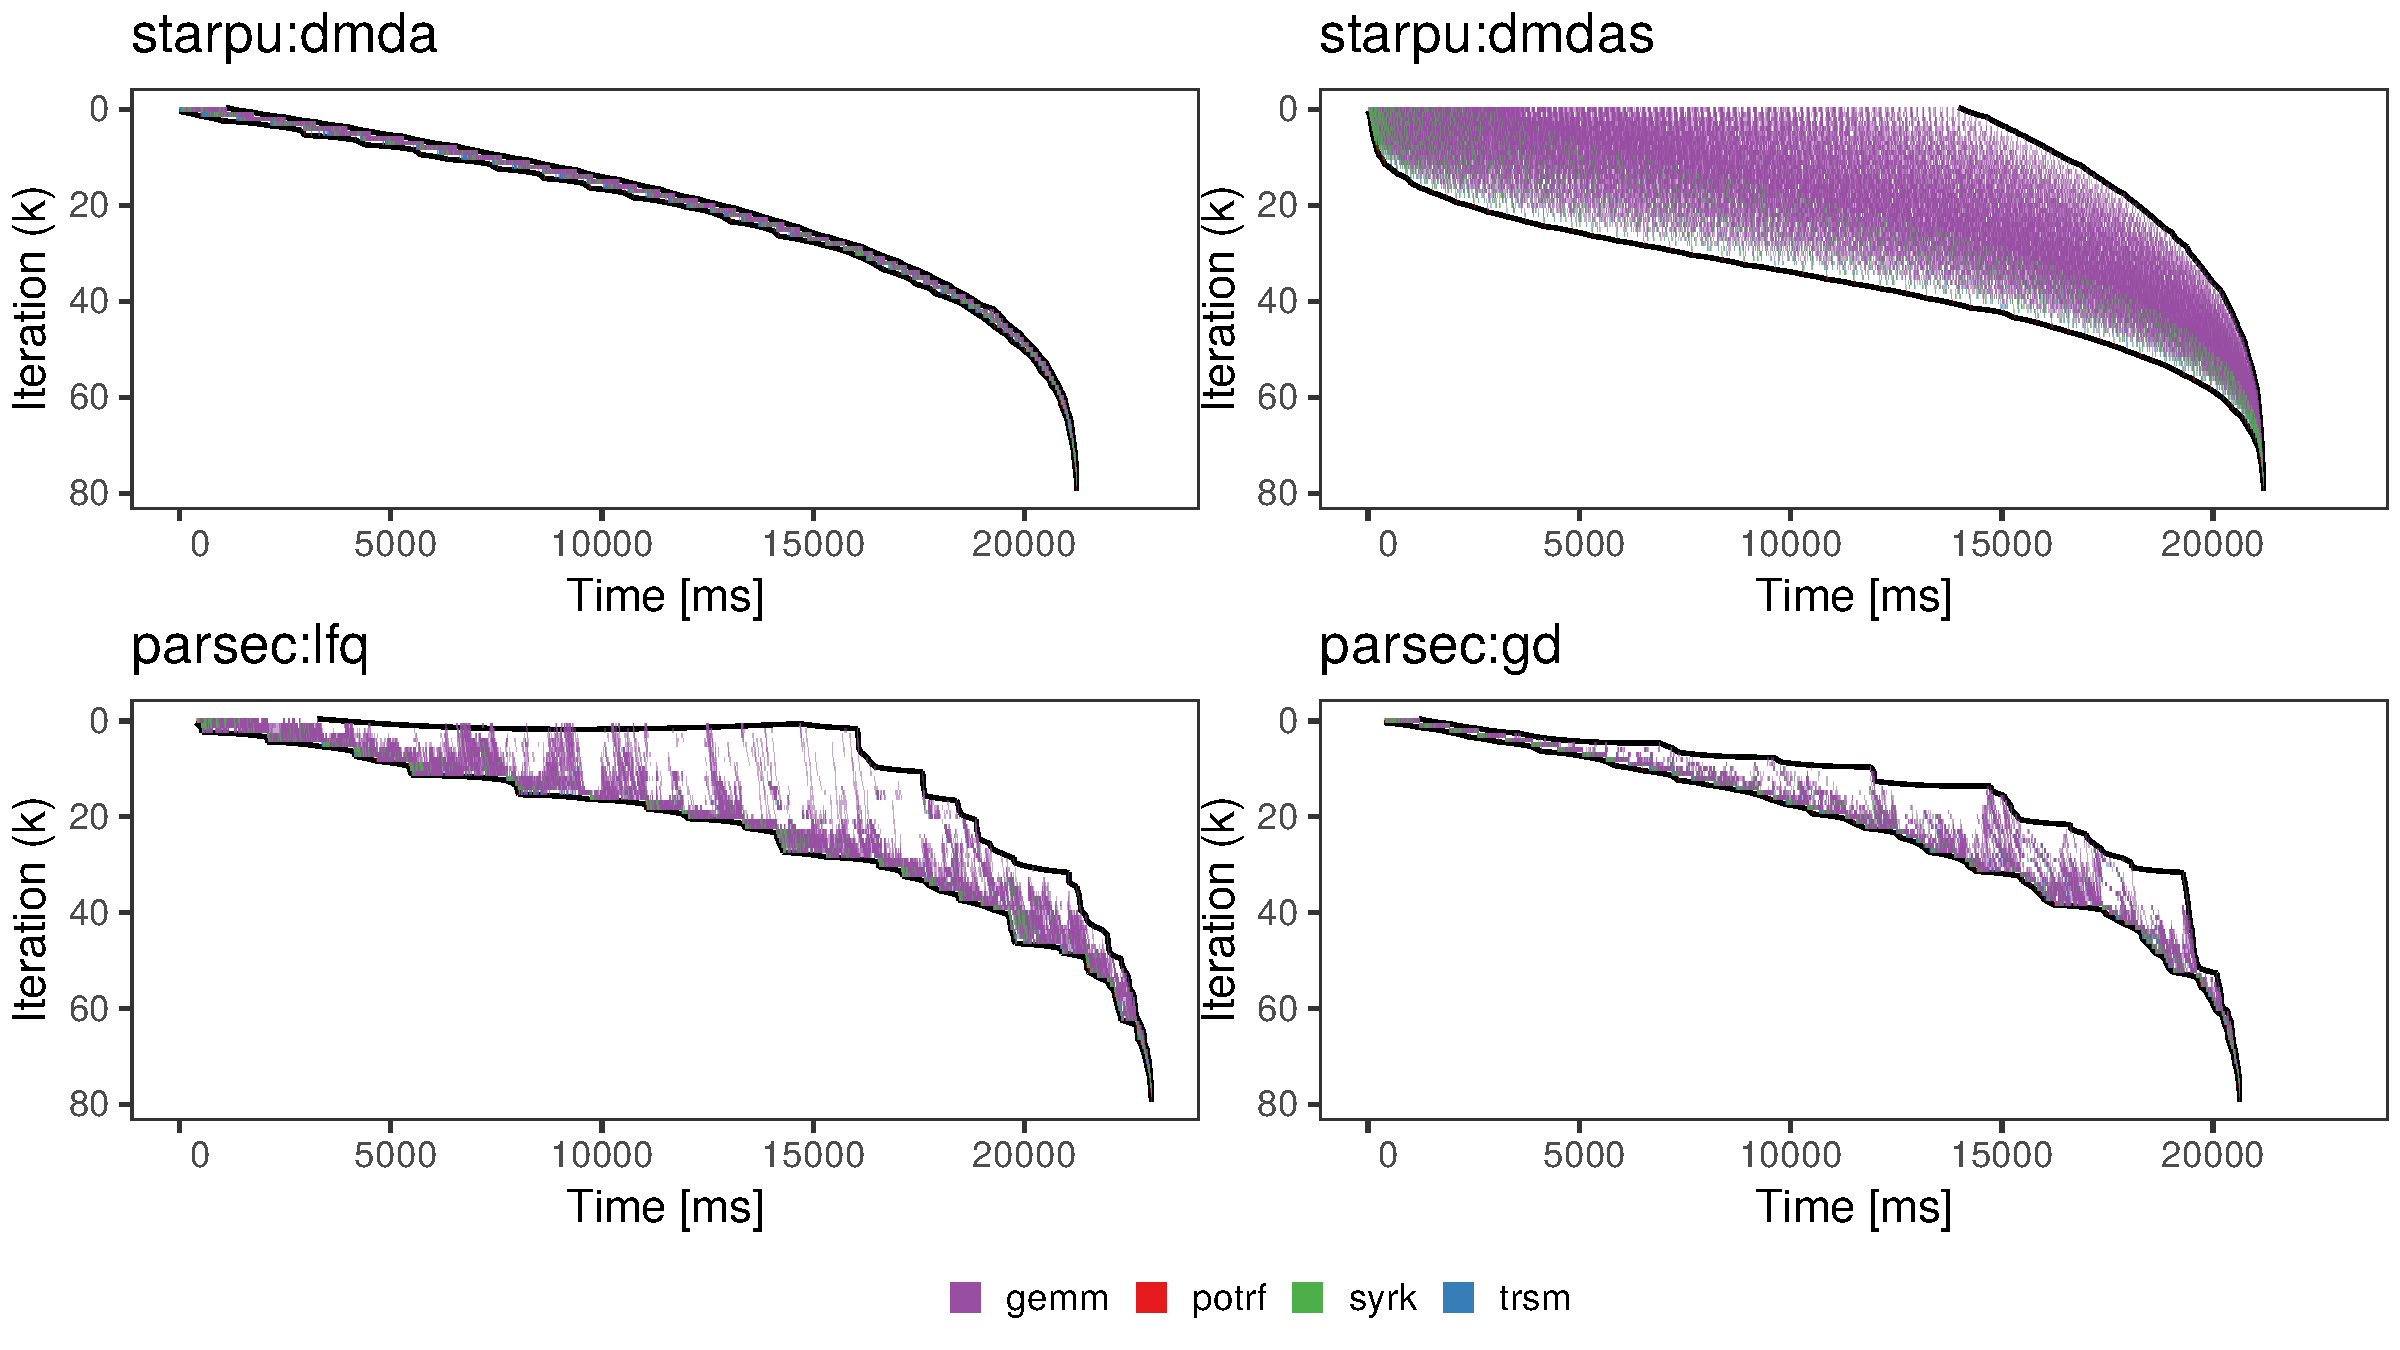
\includegraphics[width=\linewidth]{../plots/final/gpu_traces_poti_20260701_131857/kiteration_compare_dpotrf.pdf}
	\caption{Progressão das iterações da fatoração de Cholesky ao longo do
		tempo, na poti.}
	\label{fig:kiteration}
\end{figure}

\subsubsection{Transferências H2D/D2H: dois modelos de memória opostos}

A Figura~\ref{fig:transfers} mostra o volume de dados transferido entre host e device por cada configuração, medido pelos contadores nativos de cada runtime.

\begin{figure}[h]
	\centering
	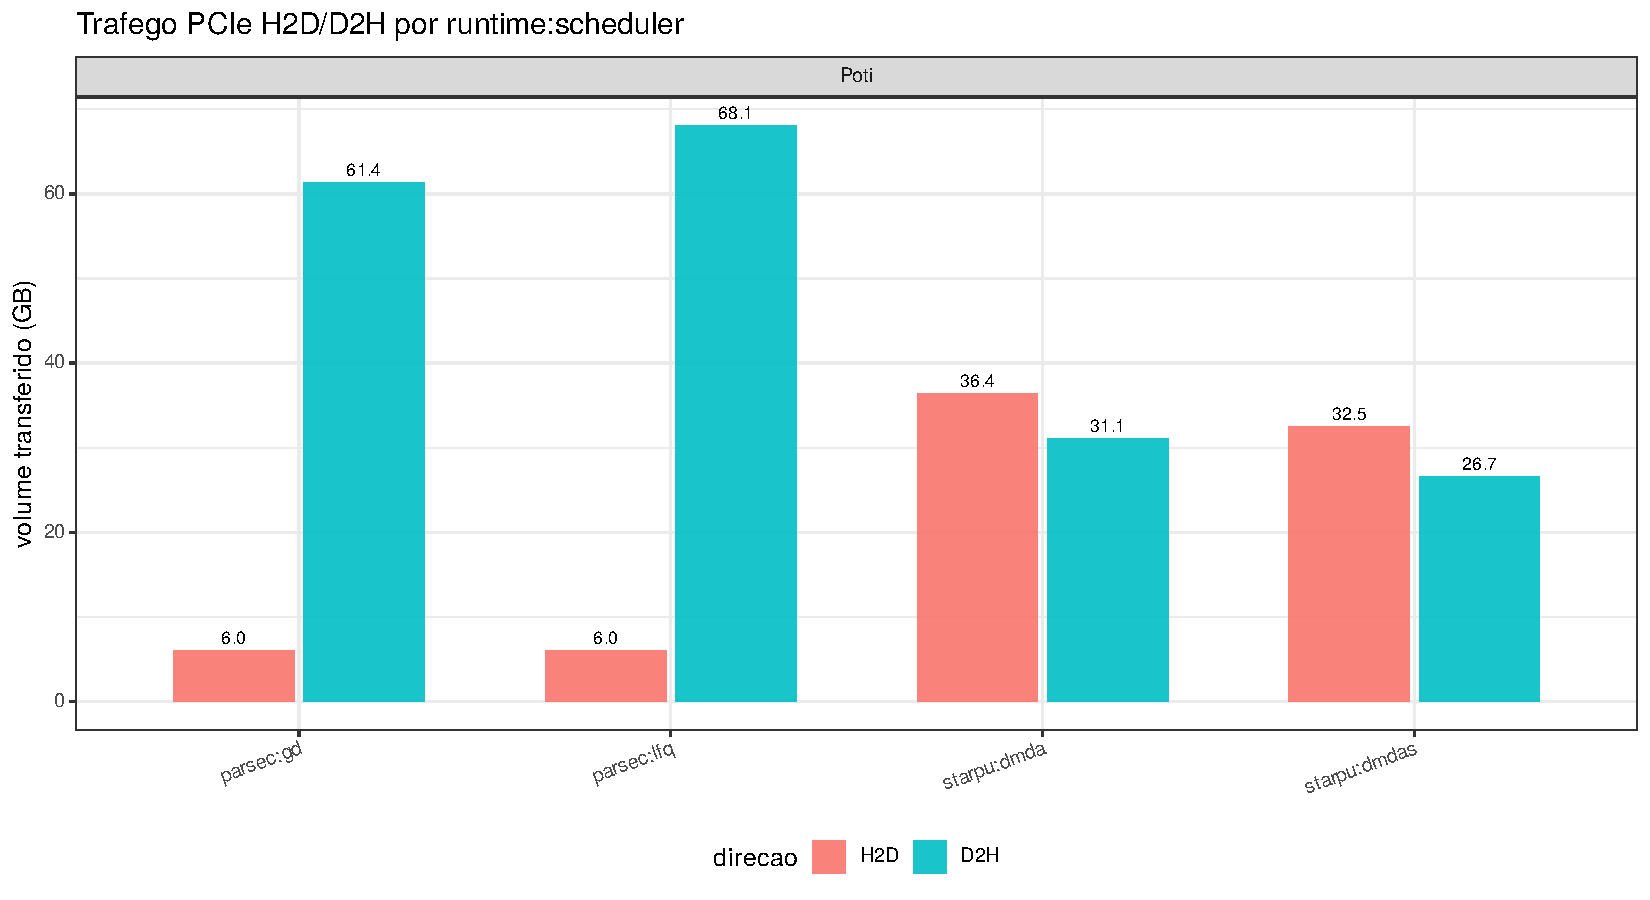
\includegraphics[width=0.7\linewidth]{../plots/final/gpu_traces_poti_20260701_131857/transfers_d2h.pdf}
	\caption{Volume de transferência H2D/D2H na poti, por configuração.}
	\label{fig:transfers}
\end{figure}

Na poti, o StarPU transfere 36,4GB H2D contra apenas 6,0GB do PaRSEC. Isso acontece pois, como a matriz em precisão dupla não cabe na VRAM da RTX 4070, o cache do StarPU envia os mesmos tiles repetidamente para a GPU. O PaRSEC quase não re-envia dados, porque a sua política de afinidade de dispositivo e seu cache seguram a maior parte dos pedidos, mas devolve ao host todo tile escrito por uma tarefa de GPU, imediatamente após a execução do kernel, o que gera um D2H muito maior. As duas direções têm custos diferentes na execução: o H2D é síncrono do ponto de vista do kernel, que só dispara quando o dado chega. O D2H do PaRSEC, por sair por um \emph{stream} dedicado e assíncrono, quase não custa tempo de computação apesar do volume maior.

\section{Conclusão}

Este trabalho comparou o desempenho dos runtimes StarPU e PaRSEC nas fatorações de Cholesky e LU sem pivotamento da biblioteca Chameleon, mantendo fixa a biblioteca de álgebra linear para isolar o efeito do runtime sobre o desempenho. Para viabilizar essa comparação, estendemos a interface DTD do PaRSEC com suporte à execução de tarefas em GPU e implementamos os codelets de GPU correspondentes no Chameleon, capacidades até então restritas ao caminho do StarPU.

Os resultados mostram que o runtime vencedor depende do equilíbrio entre a capacidade de CPU e de GPU de cada máquina. Na poti, cuja GPU é fraca em precisão dupla, o PaRSEC com o escalonador \texttt{gd} venceu por tratar a GPU como recurso adicional, sem impor custo estrutural sobre os workers de CPU. Na tupi, cuja GPU é forte, o StarPU venceu com folga por ocupá-la de forma mais eficiente, apesar do custo adicional que suas threads dedicadas à gestão da GPU impõem sobre a CPU. A análise dos rastros de execução confirmou que essa inversão ocorre por conta das diferenças entre os dois runtimes, onde o StarPU obtém maior eficiência por tarefa de GPU graças ao prefetching e ao pipelining entre host e device, mas paga por isso reservando workers de CPU à gestão da GPU. Por outro lado, o PaRSEC gerencia a GPU de forma oportunista e mais barata para a CPU, mas devolve ao host todo tile modificado por uma tarefa de GPU, gerando um volume de transferências D2H muito maior.

\bibliographystyle{sbc}
\bibliography{refs}

\end{document}
